% ENEL 617 Radio Frequency Integrated Circuits Project Report
% Pouyan Keshavarzian
% Winter 2017
% Master's of Science in Electrical Engineering studies

%-------------------------------------------------------------------------------
% DOC SETUP
\documentclass{article}                                                         % document type
\usepackage[margin=0.7in]{geometry}                                             % Set margins
\usepackage{hyperref}                                                           % Enables typesetting of hyperlinks
\usepackage{float}                                                              % Required to keep images where they are put
\usepackage[dvipsnames]{xcolor}                                                 % More colors!
\usepackage{graphicx}                                                           % Required for the inclusion of images
\usepackage{listings}                                                           % Required for the inclusion of source code
\usepackage{mathtools}                                                          % Math looks pretty. Main backbone is amsmath
\usepackage{enumitem}                                                           % Required to use different characters for enumerated lists
\usepackage{multirow}                                                           % Create tabular cells spanning multiple rows
\usepackage[toc]{glossaries}                                                    % Create glossary
\usepackage[titletoc]{appendix}                                                 % Create Appendix
\usepackage{wrapfig}                                                            % Needed for wrapping text around a figure
\usepackage{subfigure}                                                          % Subfigures
%\usepackage[]{mcode}                                                           % Matlab code
\setlength\parindent{0pt}                                                       % Removes all indentation from paragraphs
\providecommand{\e}[1]{\ensuremath{\times 10^{#1}}}                             % Use scientific notation
%\usepackage{times}                                                             % Uncomment to use the Times New Roman font
\usepackage{pdfpages}                                                           % Simplifies inclusion of external multi-page pdfs into document
\loadglsentries[main]{glossary}                                                 % Glossary
\makeglossaries
\usepackage[backend=bibtex, firstinits=false, style=ieee]{biblatex}
\addbibresource{Bibliog.bib}
\usepackage{verbatim}                                                           % Does things verbatim?? For example \verbatiminput{appendices/GuitarTunerApp.mc}. Also adds \begin{comment}. Also reporduces text verbatum
\usepackage{pdflscape}                                                          % For landscape pages
%-------------------------------------------------------------------------------
%----------------------------------------------------------------------------------------
%	DOCUMENT TITLE PAGE
%----------------------------------------------------------------------------------------
\title{\textsc{\textbf{ENEL 617 WINTER 2017 PROJECT REPORT}}} % Title
\author{\textsc{Millimeter-Wave Double Balanced Gilbert Mixer}
\\ \textsc{Pouyan Keshavarzian}}
\date{\today} % Date for the reports
\begin{document}
\maketitle % Insert the title, author and date
\newpage
%----------------------------------------------------------------------------------------
%	Table of Contents and Figures
%----------------------------------------------------------------------------------------
% Add tables and lists as required
\tableofcontents
\listoffigures
\listoftables
%-------------------------------------------------------------------------------
\newpage
%----------------------------------------------------------------------------------------
%	GLOSSARY
%----------------------------------------------------------------------------------------
\section{Glossary}
\printglossary[title=Terms Acronyms and Abbreviations]
\newpage
%----------------------------------------------------------------------------------------
%	SECTION
%----------------------------------------------------------------------------------------
\section{PROJECT MOTIVATION}
In this project, I present a double balanced mixer that would be used as part of a  BPSK Modulator circuit
to generate a spread spectrum radar waveform in the automotive frequency band (77-81 GHz). A similar modulator
that uses a double-balanced mixer is described in [CITE]. The original design benchmarks for this mixer
and the achieved final results are outlined in Table ~\ref{table:goalsnresults}.\vspace{3mm}
\vspace{3mm}
\begin{table}[H]
\centering
 \begin{tabular}{ | c | c | c |}
   \hline
    \textbf{Parameter} & \textbf{Original} & \textbf{Achieved}  \\
    \hline
    \hline
    Supply Voltage & 1.8V & 0.85V \\
    \hline
    Power Consumption & 5mW & $\approx$ \textbf{\textcolor{OliveGreen}{4.8mW}}\\
    \hline
    Gain (dB)   & 5.4 & $\approx$ \textbf{\textcolor{Red}{-13 dB}} \\
    \hline
    Input Match  & 50$\Omega$ & \textbf{\textcolor{OliveGreen}{45.5 + j0.1$\Omega$}} \\
    \hline
    Output Match & 730$\Omega$ & \textbf{\textcolor{Orange}{48.9 + j0.1$\Omega$}}\\
    \hline
    NF & 10dB & $\approx$ \textbf{\textcolor{Red}{16 dB}}\\
    \hline
    P1dB & -- & $\approx$ 1.5dB  \\
    \hline
    IP3 & -- & $\approx$ 9.5dB  \\
    \hline
  \end{tabular}
  \caption{Mixer Design Goals}
  \label{table:goalsnresults}
\end{table}
The original values were generated based on a few simple simulations/calculations and a power budget provided by Dr. Belostotski. Once the Id-gm
characteristics were understood from simulation, the gain estimate was calculated using the following equation.
\begin{equation}
  \label{eq:idealgain}
  G=\dfrac{2}{\pi}\dfrac{R_L}{R_s + \dfrac{1}{g_m}};
\end{equation}
The exact values including plots for the final results will be clearly outlined. Furthermore, deviations from original to achieved results
will be described in detail. A different design topology was used in the final design than in the original biased circuit used to calculate
the conversion gain. Some targets (such as output impedance) were changed intentionally (for practical purposes) while other values
were adjusted based on non-ideal aspects of the circuit.\vspace{3mm}
A derivation of Equation ~\ref{eq:idealgain} will be provided in the theory of operation section. A suitable value of $R_L$ was chosen
based on biasing and achieving high gain. This value, and others, deviate greatly from the final design. A thorough explanation of the
reasons for deviating are provided.
The interest in this particular-type of radar stems from spread-spectrum technology's built in interference rejection, which
is an indispensable feature for automotive radar. This type of radar has recently been demonstrated in
SiGe technology [CITE]. 65nm technology is chosen because the Figure of Merit, $f_T \approx 160GHz $, making it suitable for
this millimeter-wave application.

\subsection{Radar Theory of Operation}

\begin{wrapfigure}{r}{0.5\textwidth}
  \begin{center}
    \includegraphics[width=0.4\textwidth] {Figures/radarblock.png}
    \caption{Radar Transceiver Block Diagram}
    \label{fig:radartrans}
  \end{center}
\end{wrapfigure}
To demonstrate how this mixer could be used in a practical application, the theory of the type of radar is discussed.
A simplified block diagram of an example spread spectrum ranging system is shown in Figure ~\ref{fig:radartrans}.
The BPSK modulator is used to spread the carrier with a pseudorandom code. The parameters of the code, which govern
the LO mixing frequency, are designed to provide an adequate range resolution within the context of automotive radar.
The achievable range resolution of the radar system is related to the chip rate (mixer LO) of the code through
Equation ~\ref{eq:rangeres}.\\

\begin{equation}
  \label{eq:rangeres}
  d_{min} \leq \dfrac{c}{2f_c}
\end{equation}

Therefore to achieve a $10cm$ range resolution a chip rate of $1.5 GHz$ is chosen. The rest of the code can be designed by
choosing the appropriate length. \\
\begin{equation}
  \label{eq:codelength}
  T_{p} = \dfrac{N}{f_c}
\end{equation}
and then achievable unambiguous range of the radar becomes
\begin{equation}
  \label{eq:maxrange}
  d_{max} \leq \dfrac{c}{2T_p}
\end{equation}
Since the code is pseudorandom, the LO frequency could be any integer division of $1.5GHz$ i.e $0.75GHz, 0.5GHz$ etc.
For the purposes of design we will simulate with just a $1.5GHz$ signal to demonstrate the maximum bandwidth of operation.
\newpage
\section{Mixer Theory of Operation}
\subsection{Basic Principle}

The Gilbert Cell is a linear time-varying circuit. The concept behind this circuit is intuitive. The RF transistors act as
transconductance amplifiers which change the input voltage to a current. The differential ports act as switches that commutate the output.
This creates the time-domain multiplication function. FIGURES X DEMOSTRATE THIS CONCEPT.

\subsection{Detailed Analysis}


\newpage
\begin{landscape}

\section{Design Variations and Final Circuit Schematic}
\subsection{Circuit Schematic}

\begin{figure}[H]
  \centering
  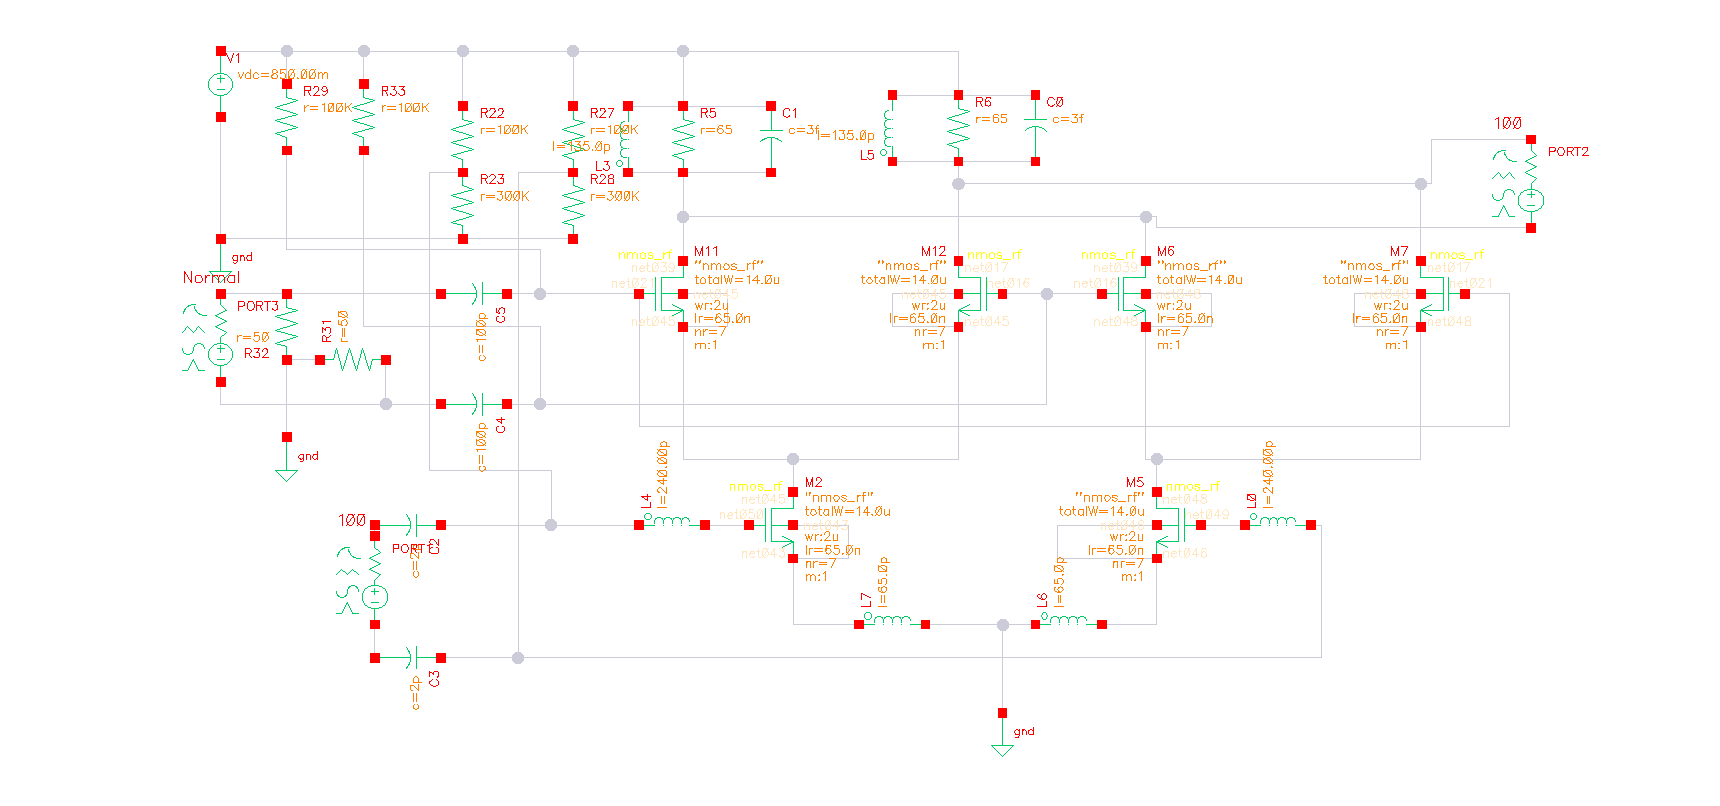
\includegraphics[width=1.5\textwidth] {Figures/Circuit.png}
  \caption{Final Design}
    \label{fig:finalschem}
\end{figure}
\end{landscape}

\newpage
\section{Simulated Results}
\subsection{Transistor Biasing and Power Consumption}
\subsection{Conversion Gain}
\begin{figure}[H]
  \centering
  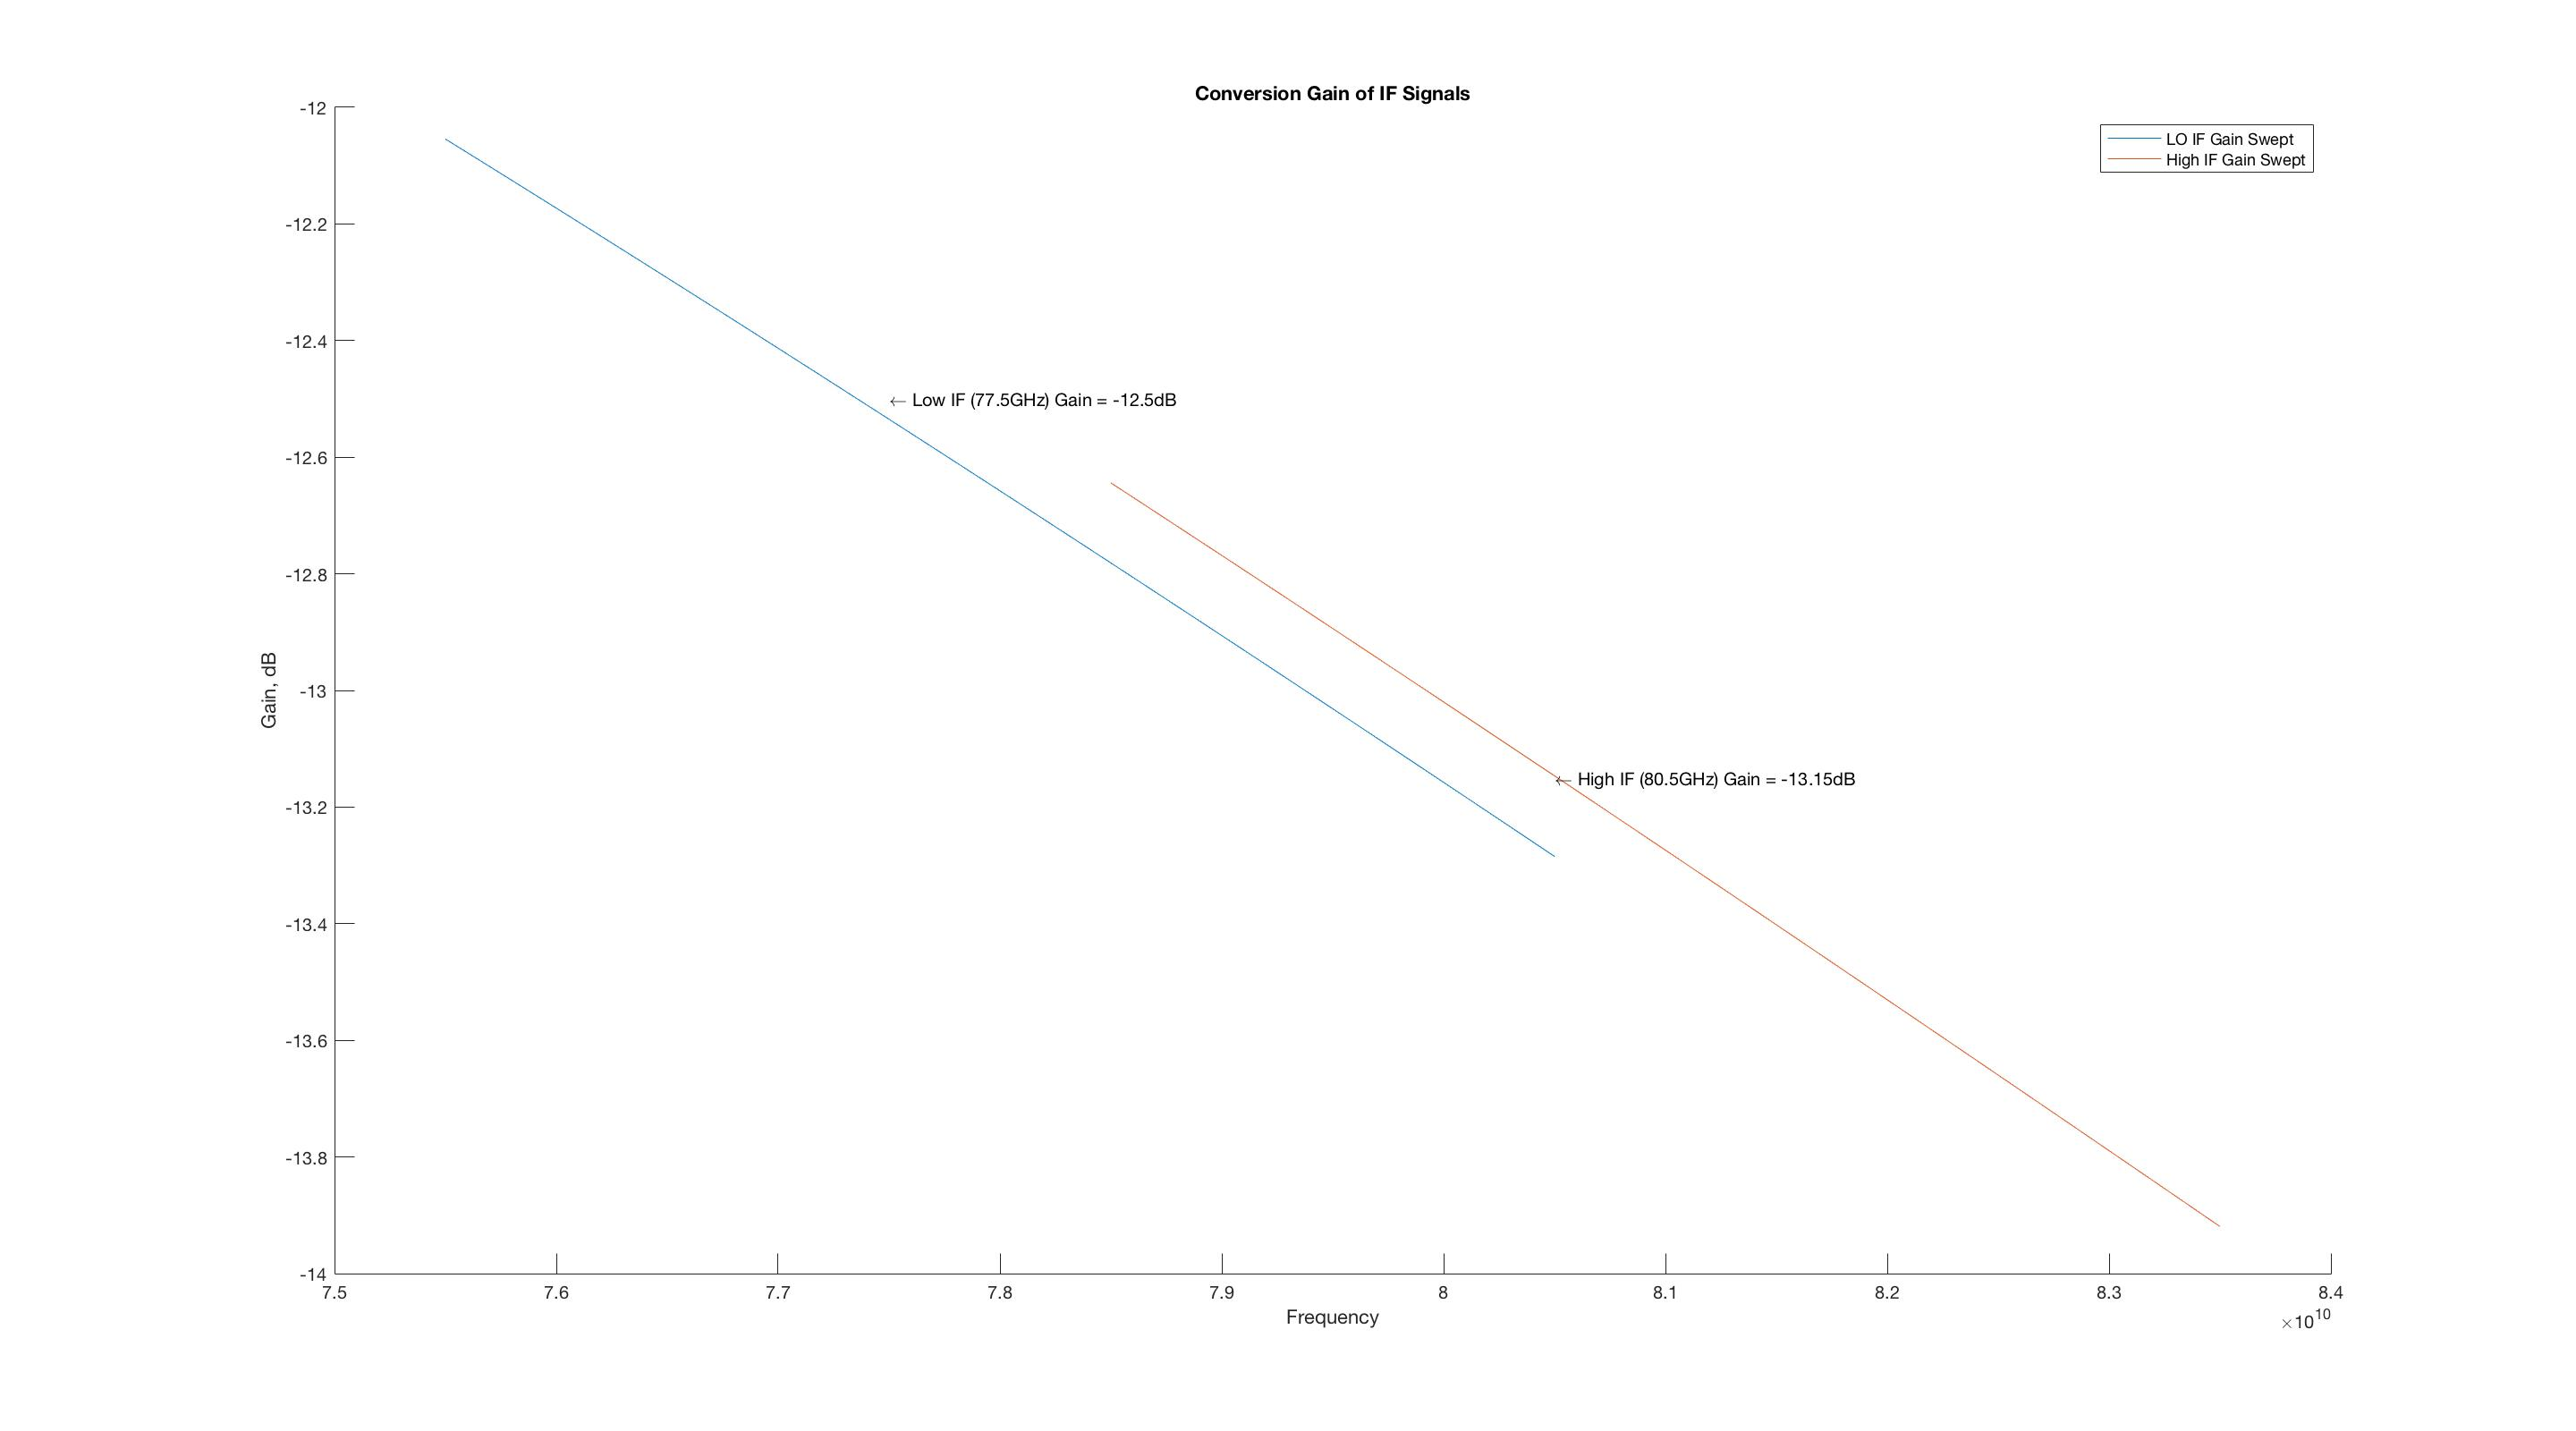
\includegraphics[width=0.95\textwidth] {Plots/Gain.jpg}
  \caption{Swept Gain for Lo and Hi IF}
    \label{fig:matgain}
\end{figure}
\subsection{Input and Output Matching}
\begin{figure}[H]
  \centering
  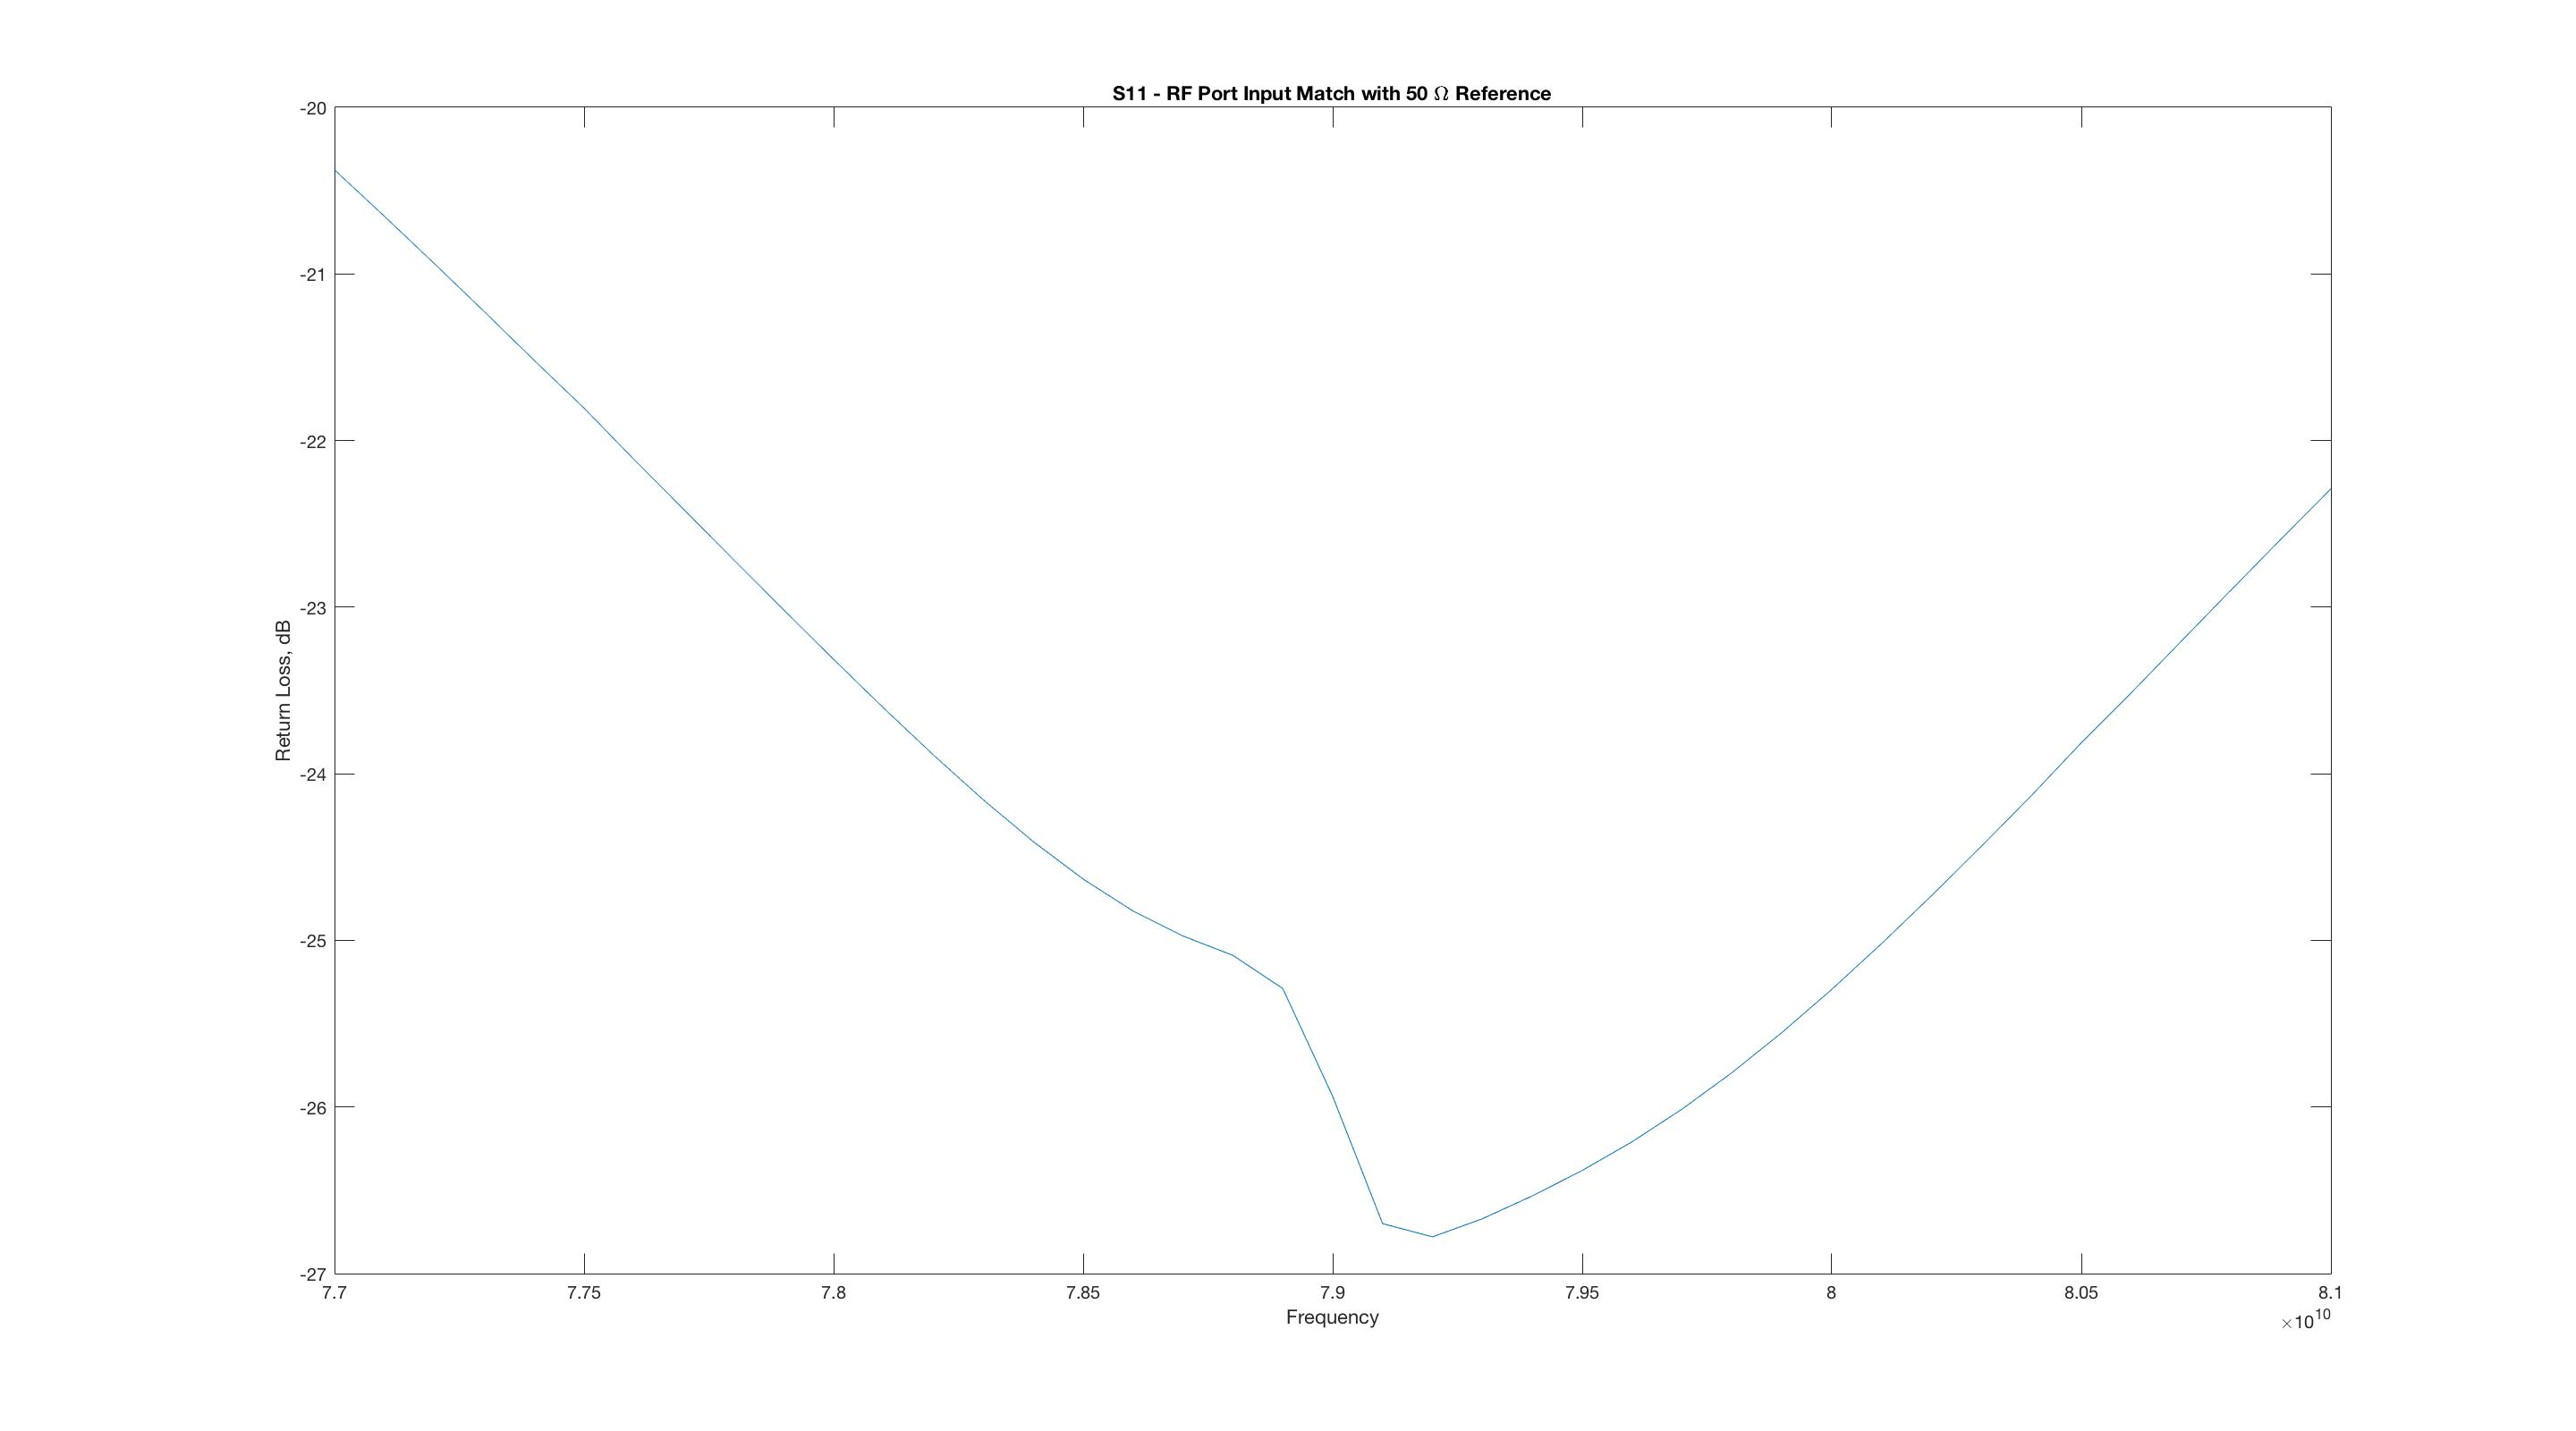
\includegraphics[width=0.95\textwidth] {Plots/S11.jpg}
  \caption{Final Return Loss of RF Port}
    \label{fig:matS11}
\end{figure}
\begin{figure}[H]
  \centering
  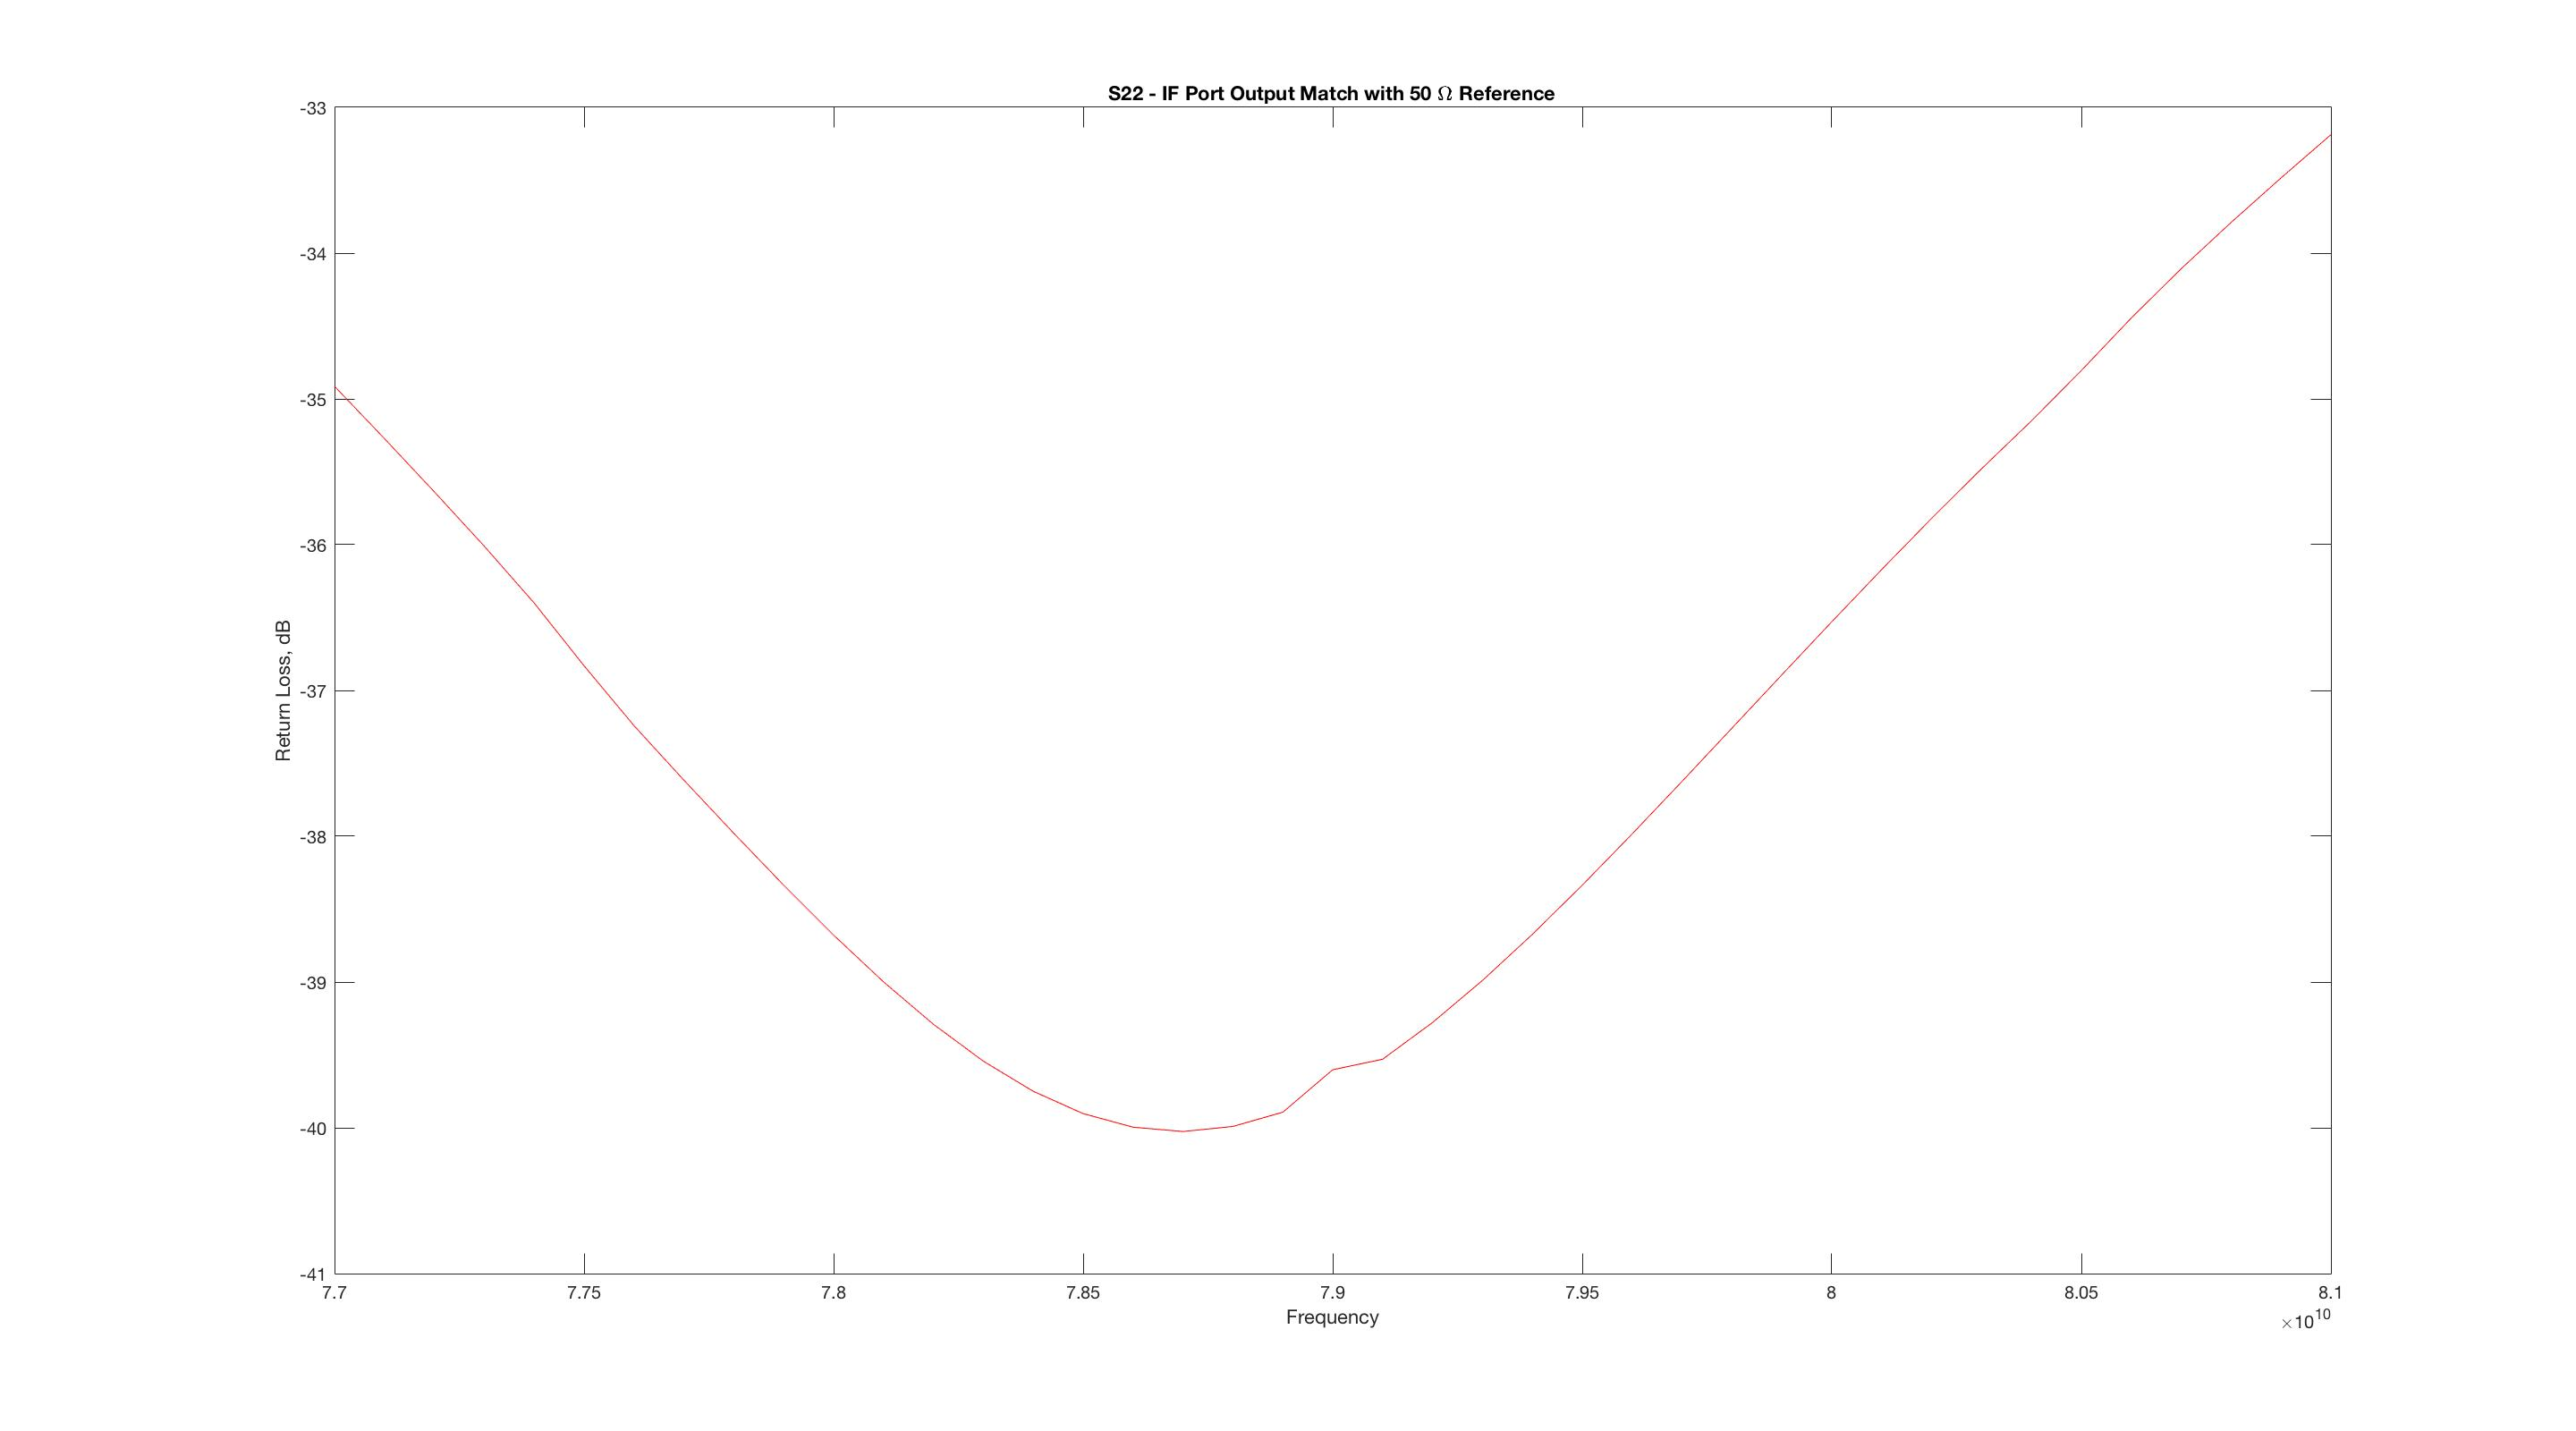
\includegraphics[width=0.95\textwidth] {Plots/S22.jpg}
  \caption{Final Return Loss of IF Port}
    \label{fig:matS11}
\end{figure}

\subsection{Noise Figure}
\begin{figure}[H]
  \centering
  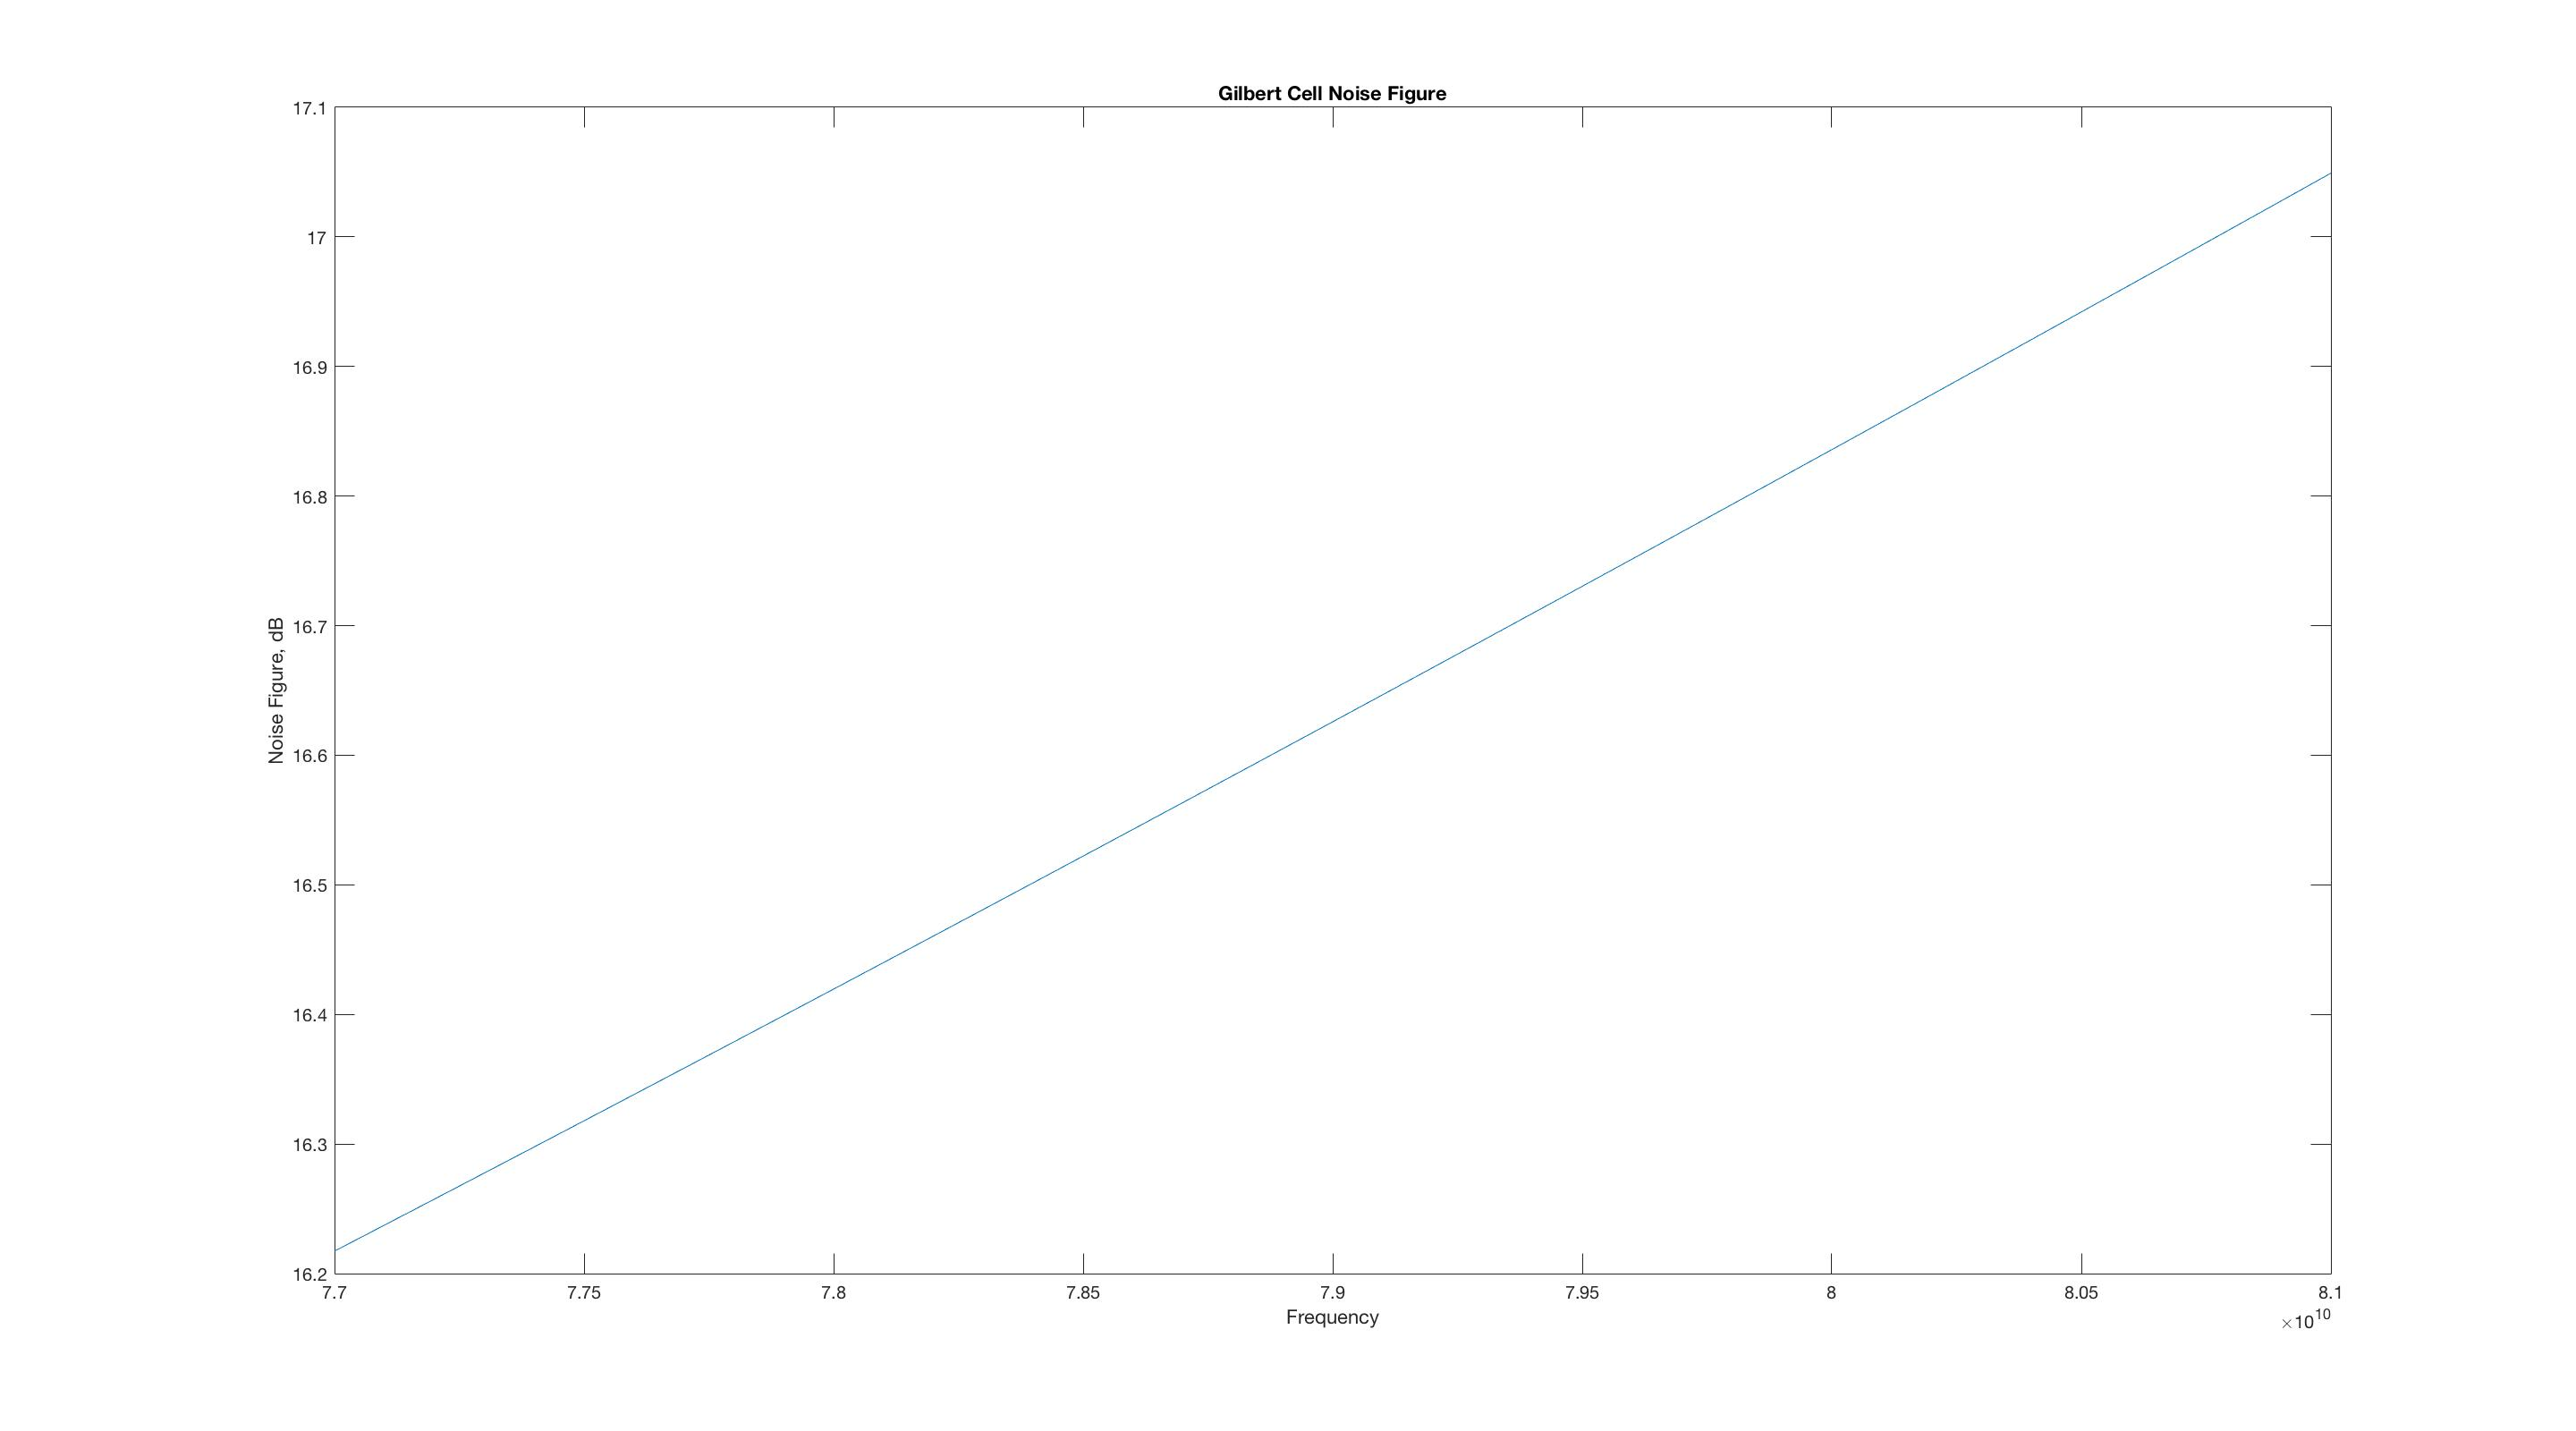
\includegraphics[width=0.95\textwidth] {Plots/NF.jpg}
  \caption{Final NF}
    \label{fig:matNF}
\end{figure}

\subsection{P1dB \& IP3}
Write some stuff about this... 
\newpage
\section{Discussion}

%----------------------------------------------------------------------------------------
%	REFERENCES
%----------------------------------------------------------------------------------------
\section{References}
\printbibliography[heading=none]

\newpage
%----------------------------------------------------------------------------------------
%	APPENDIX
%---------------------------------------------------------------------------------------
\begin{appendices}
\section{Cadence Simulation Plots}\label{app:cresults}
\subsection{Conversion Gain}
\begin{figure}[H]
  \centering
  \includegraphics[width=0.95\textwidth] {Figures/FinalConversionGain.bmp}
  \caption{Conversion Gain Cadence}
    \label{fig:cGain}
\end{figure}
\subsection{RMS Spectrum}
\begin{figure}[H]
  \centering
  \includegraphics[width=0.95\textwidth] {Figures/FinalSpectrum.bmp}
  \caption{RMS Spectrum Cadence}
    \label{fig:cSpectrum}
\end{figure}
\subsection{Noise Figure}
\begin{figure}[H]
  \centering
  \includegraphics[width=0.95\textwidth] {Figures/FinalNF.bmp}
  \caption{Noise Figure Cadence}
    \label{fig:cNF}
\end{figure}
\subsection{P1dB}
\begin{figure}[H]
  \centering
  \includegraphics[width=0.95\textwidth] {Figures/P1dB_GOOD_ATTEMPT1_77point5.bmp}
  \caption{P1dB Cadence}
    \label{fig:cP1db}
\end{figure}
\subsection{IP3}
\begin{figure}[H]
  \centering
  \includegraphics[width=0.95\textwidth] {Figures/IP3dB_GOOD_ATTEMPT1.bmp}
  \caption{IP3 Cadence}
    \label{fig:cIP3}
\end{figure}
\subsection{S11}
\begin{figure}[H]
  \centering
  \includegraphics[width=0.95\textwidth] {Figures/FinalS11_rect.bmp}
  \caption{RF Port Match}
    \label{fig:cS11}
\end{figure}
\subsection{S22}
\begin{figure}[H]
  \centering
  \includegraphics[width=0.95\textwidth] {Figures/FinalS22Rect.bmp}
  \caption{IF Port Match}
    \label{fig:cS22}
\end{figure}


\end{appendices}

\end{document}
